\let\negmedspace\undefined
\let\negthickspace\undefined
\documentclass[journal]{IEEEtran}
\usepackage[a5paper, margin=10mm, onecolumn]{geometry}
\usepackage{lmodern} 
\usepackage{tfrupee} 
\setlength{\headheight}{1cm}
\setlength{\headsep}{0mm}   

\usepackage{gvv-book}
\usepackage{gvv}
\usepackage{cite}
\usepackage{amsmath,amssymb,amsfonts,amsthm}
\usepackage{algorithmic}
\usepackage{graphicx}
\usepackage{textcomp}
\usepackage{xcolor}
\usepackage{txfonts}
\usepackage{listings}
\usepackage{enumitem}
\usepackage{mathtools}
\usepackage{gensymb}
\usepackage{comment}
\usepackage[breaklinks=true]{hyperref}
\usepackage{tkz-euclide} 
\usepackage{listings}                             
\def\inputGnumericTable{}                                 
\usepackage[latin1]{inputenc}                                
\usepackage{color}                                            
\usepackage{array}                                            
\usepackage{longtable}                                       
\usepackage{calc}                                             
\usepackage{multirow}                                         
\usepackage{hhline}                                           
\usepackage{ifthen}                                           
\usepackage{lscape}
\usepackage{xparse}

\bibliographystyle{IEEEtran}

\title{2.5.30}
\author{EE25BTECH11062 - Vivek K Kumar}

\begin{document}
\maketitle

\renewcommand{\thefigure}{\theenumi}
\renewcommand{\thetable}{\theenumi}

\numberwithin{equation}{enumi}
\numberwithin{figure}{enumi} 

\textbf{Question}:\\
If the two Lines 
\begin{align}
    L_1 &: x=5, \frac{y}{3-\alpha} = \frac{z}{-2} \text{ and} \\
    L_2 &: x=2, \frac{y}{-1} = \frac{z}{2-\alpha}
\end{align}
are perpendicular, then the value of $\alpha$ is \underline{\hspace{0.1\columnwidth}}
\\
\textbf{Solution: }
\begin{table}[H]    
  \centering
  \begin{table}[h!]
    \centering
    \begin{tabular}{|c|c|}
        \hline
        Point & Coordinates \\
        \hline
	    $A$ & $\myvec{1\\-1}$ \\
	    $B$ & $\myvec{-4\\2k}$ \\
	    $C$ & $\myvec{-k\\-5}$ \\
        \hline
    \end{tabular}
    \caption{Vertices of $\triangle ABC$ before substituting $k$}
    \label{tab:triangle_k}
\end{table}

  \caption{Variables Used}
  \label{tab:2.5.30}
\end{table}
The lines can be represented as\\
\begin{align}
\vec{x} &= \myvec{5\\0\\0} + \kappa_1\vec{m_1}\\
           &= \myvec{5\\0\\0} + \kappa_1\myvec{0\\3-\alpha\\-2}
\end{align}
and 
\begin{align}
\vec{x} &= \myvec{2\\0\\0} + \kappa_2\vec{m_2}\\
           &= \myvec{2\\0\\0} + \kappa_2\myvec{0\\-1\\2-\alpha}
\end{align}

As the given lines are perpendicular, their direction vectors follow the relation: 
\begin{align}
    \vec{m_1}^T\vec{m_2} = 0 \\
    \myvec{0&3-\alpha&-2}\myvec{0\\-1\\2-\alpha} = 0\\
    3\alpha - 7 = 0\\
    \text{which gives } \alpha = \frac{7}{3}\\
    \text{and } \vec{m_1} = \myvec{0 \\ \frac{2}{3} \\ -2} , \vec{m_2} = \myvec{0 \\ -1 \\ \frac{-1}{3}}
\end{align}
\begin{figure}[H]
   \centering
  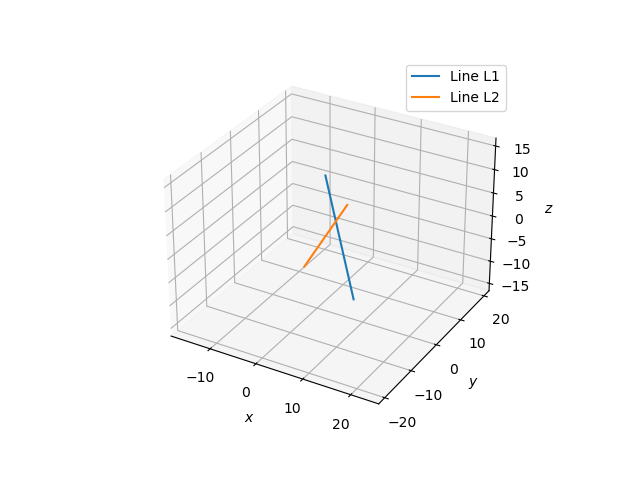
\includegraphics[width=0.64\columnwidth]{figs/fig.png}
   \caption{Given vector and its direction cosines}
   \label{stemplot}
\end{figure}
\end{document}  

